\chapter{Non-Relational Database} 

Relational database has been introduced in the earlier chapter. This chapter discusses non-relational database.

\section{Brief Introduction to Non-Relational Database}

Non-relational databases (NoSQL databases) gained its popularity in the $2000$s. In contrast to RDB, NoSQL databases do not store data in tables the way RDB does, but in key-value pairs, graphs, documents, or other formats, and it is more flexible, efficient and easier to use in some applications than the conventional RDBs. Examples of NoSQL databases include \textit{Redis}, \textit{Azure CosmosDB}, \textit{Oracle NoSQL Database}, \textit{Amazon DynamoDB}, \textit{MongoDB}, \textit{AllegroGraph} and many more.

Unlike SQL which applies to almost all RDBMS, there is no universally adopted language for NoSQL DBMS. Each NoSQL database often has its unique query language tailored to its specific data model. We use ``NoSQL'' to refer to a collective set of languages used for NoSQL database management. For simple applications, different RDB may perform similarly, with some subtle differences in the performance. However, this is different for NoSQL databases, which may function completely differently.

There are many types of non-relational databases including document-oriented databases, directed graph databases, etc. Each of them has some unique features over other databases, and may adopt its own database manipulation language. It is impossible to cover everything in this notebook. Only brief introductions of selected databases examples are given here. More details might be found on other relevant notebooks, for example graphical database in \textit{A Notebook on Probability, Statistics and Data Science} as part of the semantic web.

Database services, both RDB and NoSQL, have become critical to our daily life and they are massively deployed on servers. In many applications they work together to deliver the service.

\section{Non-RDB Example: MongoDB}

MongoDB is a source-available, cross-platform, general-purpose, document-oriented database program. Classified as a NoSQL database program, MongoDB uses BSON (an extension of JSON) documents with flexible schema to store data. This is not surprising, as MongoDB itself is powered by a JavaScript engine. MongoDB, together with other JavaScript-relevant software such as \textit{Express.js}, \textit{React.js}, \textit{Node.js}, etc., is often used to create database-powered web applications.

Data in MongoDB can be exported or imported from files, such as BSON and JSON files.

\subsection{Features of MongoDB}

Comparing with conventional RDBs, MongoDB is better at
\begin{itemize}
	\item Massive data storage (in the order of TBs and PBs);
	\item Frequent and parallel operations when performing insert and query;
	\item Flexible scalability and high availability.
\end{itemize}
Notice that MongoDB as well as many other NoSQL databases are not suitable to handle financial transactions due to the consistency issue that many NoSQL databases suffer. But things might change as new technologies become handy.

Examples of MongoDB-suitable applications include
\begin{itemize}
	\item Posts and streaming management on social media websites or APPs;
	\item Online gaming;
	\item Logistics industry and supply chain management;
	\item IoT data management.
\end{itemize}

As a document-oriented database, MongoDB stores data in documents and collections instead of rows and tables. A document is the basic unit of the storage. A collection is a group of documents on the same/similar topic. Each document in the same collection can adopt its own schema, and it should be self-contained so that when querying the data the user does not need to join collections and map documents. Figure \ref{ch:database:mongotree} gives a demonstrative example of how MongoDB stores and organizes data.
\begin{figure}[htbp]
	\centering
	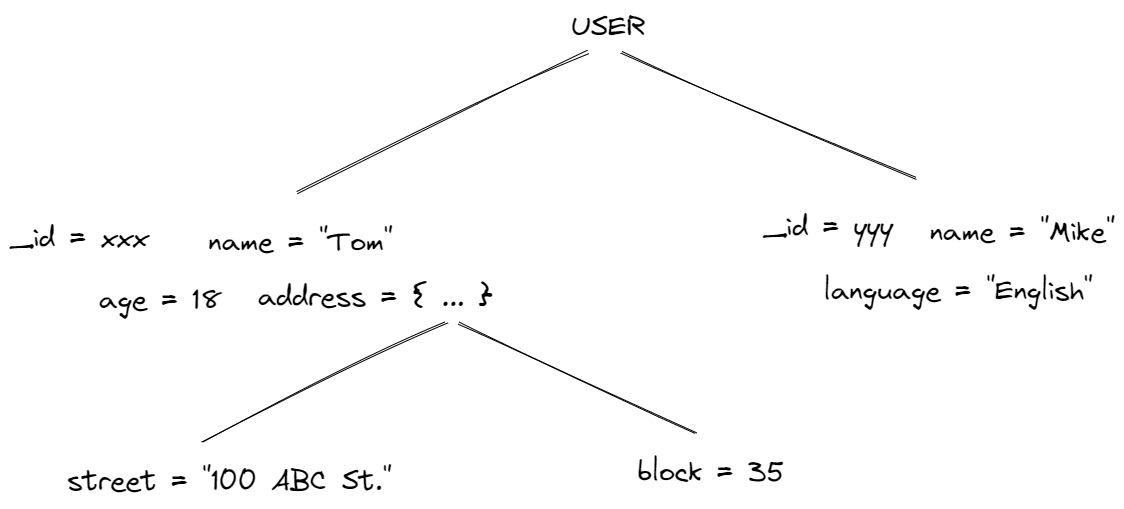
\includegraphics[width=250pt]{chapters/part-3/figures/mongodb_tree.png}
	\caption{A demonstrative example of how MongoDB stores data as (nested) object.} \label{ch:database:mongotree}
\end{figure}

In Fig. \ref{ch:database:mongotree}, a collection ``USER'' is defined. The collection contains two documents. Each document has a few properties. Different document may share common properties such as ``name'' in this example. Each of them can also have unique properties of its own such as ``age'', ``address'' and ``language''. Different properties may have different data types. For example, a property can be string, numeric, or a nested object, or an array of the above. When querying MongoDB, the DBMS is able to return selected properties of documents that meet specific criteria, and sort them in the required order.

\subsection{Data Format in MongoDB}

MongoDB is a document-oriented database program. The data is stored in the format of ``binary JSON'' known as BSON. BSON is an extension of JSON that supports more data types.

\begin{shortbox}
	\Boxhead{JSON VS BSON}
	
	JSON supports the following 6 data types: number, string, boolean, object, array, and null. JSON is text-based, which means that it is essentially a string. It is only a notation of data and does not concern itself with how the data is interpreted in the program that processes the JSON file. For example, ``0'' as a number in a JSON file does not imply whether it is an integer, a 32-bit float, or a 64-bit float.
	
	BSON, on the other hand, is binary-based and hence contains more information. In BSON, more data types are supported, such as different floats, date, timestamp, binary string, regular expression, code, etc. For the same example, ``0'', in BSON different number types are compiled and stored differently. This makes BSON more powerful and efficient (but less intuitive) than JSON.
	
\end{shortbox}

MongoDB uses BSON to store and process data due to its enhanced capability, and uses JSON to display the data.

\subsection{Installation}

MongoDB, like many other DBMS, has both community and enterprise versions. MongoDB community server can be installed following the instructions in the official website
\begin{lstlisting}
https://www.mongodb.com/try/download/community
\end{lstlisting}
A MongoDB server can host a MongoDB cluster, inside which are many MongoDB databases. Each database can have its own access policy, etc.

To interact with MongoDB DBMS, the quickest way is to use MongoDB shell (also known as ``mongosh''). A description of the shell can be found at
\begin{lstlisting}
https://www.mongodb.com/try/download/shell
\end{lstlisting}
Notice that when installing MongoDB server, it is possible that the server comes with MongoDB Compass, the GUI for MongoDB DBMS. The GUI can also be used to interact with the databases.

Different versions of MongoDB are available. Choose the correct MongoDB version depending on the CPU and the OS of the machine. MongoDB community server installation size is about 500MB.

MongoDB provides enterprise service, MongoDB Atlas, as part of its cloud solution where user can deploy clusters to host databases. With proper gateway setup, the user can connect to MongoDB Atlas clusters from his local server to retrieve data or to manipulate the databases. MongoDB Atlas is briefly introduced in a later section.

\subsection{MongoDB Shell}

After installing both MongoDB server and MonghDB shell, use
\begin{lstlisting}
$ mongosh
\end{lstlisting}
in the command line to login to the DBMS. JavaScript-like commands are used to manipulate the database, such as creating databases and inserting data.

\vspace{0.1in}
\noindent \textbf{Basic Operation}
\vspace{0.1in}

The object \verb|db| contains many methods using which the user can access and modify the basic configurations of the database. For example,
\begin{lstlisting}
> db.version()
\end{lstlisting}
gives the version of the database server. More commands can be found using \verb|db.help()|. Some commonly used commands are listed in Table \ref{ch:db:tab:mongodbbasics}.
\begin{table}
	\centering \caption{MongoDB basic commands.}\label{ch:db:tab:mongodbbasics}
	\begin{tabularx}{\textwidth}{lX}
		\hline
		Command & Description \\ \hline
        \verb|db.help()| & Show a list of methods of \verb|db| object. \\ 
		\verb|db.version()| & Show database server version. \\ 
        \verb|db.getUsers()| & Show users. \\ 
        \verb|db.createUser(<content>)| & Create a user. The username, password, roles, etc., needs to be included in the \verb|<content>| area. \\ 
        \verb|db.dropUser(<username>)| & Drop a user. \\ 
        \verb|db.dropDatabase()| & Drop current database. \\ 
		\verb|db.status()| & Show the basic status of the currently selected database, such as its name, number of collections, storage size, etc.  \\
		 \hline
	\end{tabularx}
\end{table}

To display the existing databases, use
\begin{lstlisting}
> show dbs
\end{lstlisting}
On a clean installation, the above should return the 3 default databases, \verb|admin|, \verb|config| and \verb|local|. To switch to a particular database, use
\begin{lstlisting}
> use <database_name>
\end{lstlisting}
Notice that there is no ``create database'' command in MongoDB. To create a database, switch to that database using the above command (even though it does not exist yet), and add some data. The database will be automatically created. This is again a feature closely related to JavaScript.

\vspace{0.1in}
\noindent \textbf{Create Collection and Document}
\vspace{0.1in}

A MongoDB database contains multiple collections. A collection is similar to a table in an RDB in the sense that it is the collection of data on the same / similar topic. However, unlike tables where schematics such as column names and datatypes are enforced upon creation of the table, a collection does not enforce fields and data types. An example of creating a collection inside a database is given below.
\begin{lstlisting}
> use testdb;
> db.createCollection("users");
\end{lstlisting}
Use \verb|show collections| to show the collections in the current database.

\begin{shortbox}
\Boxhead{Should I use semicolon in the end of each MongoDB command?}

If you are using MongoDB shell, then technically speaking, you don't have to. It works both ways. However, if you are using JavaScript environment such as \textit{Node.js} and integrating MongoDB commands as part of the program, you should use semicolon.

For example, to create a new database, in MongoDB shell
\begin{lstlisting}
> use myNewDatabase
\end{lstlisting}
or
\begin{lstlisting}
> use myNewDatabase;
\end{lstlisting}
would both work just fine. However, in \textit{Node.js},
\begin{lstlisting}
const newDb = client.db("myNewDatabase");
\end{lstlisting}
the semicolon is required by the JavaScript syntax.

As a conclusion, semicolon is recommended mostly, just to follow the general JavaScript good practice. Although in JavaScript semicolon is also optional due to Automatic Semicolon Insertion (ASI), it is still widely recommended to use semicolon anyway.
\end{shortbox}

Data can be inserted into a collection in the form of documents. It is possible to insert one or multiple documents at a time. To insert documents, first prepare the document in JSON-like format. For example, consider the following documents.
\begin{lstlisting}
{
  name: "Alice",
  age: 20,
  address: "123 Center Park",
  hobbies: ["football", "reading"],
  parents: {
    father: "Chris",
    mother: "Kite"
  }
}

{
  name: "Bob",
  age: Long.fromNumber(25),
  address: "135 Center Park",
  hobbies: BSON.Array(["basketball", "jogging"])
}
\end{lstlisting}
Notice that user ``Alice'' and ``Bob'' are represented by JSON and BSON, respectively. MongoDB uses BSON internally, but it can also take JSON as input, in which case MongoDB driver converts JSON to BSON.

Then use the following syntax to insert the document into the collection.
\begin{lstlisting}
db.<collection_name>.insertOne({...});
db.<collection_name>.insertMany([{...}, {...}, {...}]);
\end{lstlisting}
where \verb|{...}| is the document in JSON or BSON format as shown earlier. To make it more readable, consider do the following instead.
\begin{lstlisting}
const doc = {...};
db.<collection_name>.insertOne(doc);
\end{lstlisting}
which first store the document in \verb|doc|, then pass it to \verb|insertOne()| method. Upon successful insertion, an insert id (also known as object id) will be created automatically.

Notice that the above inserting document method creates a collection, if the collection has not been created.

The field \verb|_id| represents the object ID, and it is compulsory for each document, and it must be unique among the documents under the same collection. If \verb|_id| is not specified when inserting the document, the system will create an object ID for that document. 

\vspace{0.1in}
\noindent \textbf{Query}
\vspace{0.1in}

MongoDB uses \verb|find({...})|, \verb|findOne({...})| to find documents, where \verb|{...}| is a query argument (filtering criteria) in the form of JavaScript object. Details are given below.

To obtain all the document under a collection, use
\begin{lstlisting}
db.getCollection('<collection_name>').find({});
\end{lstlisting}
where an empty query simply matches all documents in the collection. Of course, when \verb|findOne()| is used, it will return only one document.

Notice that
\begin{lstlisting}
db.<collection_name>.<function>()
\end{lstlisting}
is equivalent with
\begin{lstlisting}
db.getCollection('<collection_name>').<function>();
\end{lstlisting}
The first implementation is more convenient while the second more flexible as it supports dynamic naming.

More examples are given below. Assume that there is a collection \verb|posts|, inside which are documents recording the posts by a blogger. Each post may have some comments. The number of comments are recorded in the field \verb|comments| of the documents. To find documents that has a certain field with certain values, use the following
\begin{lstlisting}
db.getCollection('posts').find({comments: 1})
\end{lstlisting}
The above query search documents with field \verb|comments| whose value is $1$ (or whose value is an array that contains $1$ as its element). under collection \verb|posts|. To get those posts with at least $1$ comment, use the following
\begin{lstlisting}
db.getCollection('posts').find({comments: {$gt: 0}})
\end{lstlisting}
where \verb|{$gt: 0}| stands for any value greater than $0$. Commonly seen query operators are given in Table \ref{ch:db:tab:mongodbqueryoperator}, each with an example.

\begin{table}
	\centering \caption{MongoDB basic query operators.} \label{ch:db:tab:mongodbqueryoperator}
	\begin{tabularx}{\textwidth}{llX}
		\hline
		Operator & Description & Example \\ \hline
		\verb|$eq| & Equal & \verb|{age: {$eq: 18}}| \\ 
		\verb|$gt| & Greater than & \verb|{age: {$gt: 18}}| \\ 
		\verb|$gte| & Greater or equal & \verb|{age: {$gte: 18}}| \\ 
		\verb|$lt| & Less than & \verb|{age: {$lt: 18}}| \\ 
		\verb|$lte| & Less or equal & \verb|{age: {$lte: 18}}| \\ 
		\verb|$and| & And & \verb|{$and: [{age: {$gt: 18}}, {sex: 'M'}]}| \\ 
		\verb|$or| & Or &  \verb|{$or: [{age: 18}, {age: 21}]}| \\ 
		\verb|$in| & In & \verb|{name: {$in: ['Alice', 'Bob']}}| \\ 
		\verb|$nin| & Not in & \verb|{name: {$nin: ['Alice', 'Bob']}}| \\
		\hline
	\end{tabularx}
\end{table}

To specifically query for elements in an array, use \verb|$elemMatch| as follows.
\begin{lstlisting}
{ <field>: { $elemMatch: { <query1>, <query2>, ... } } }
\end{lstlisting}
For example,
\begin{lstlisting}
db.scores.find(
	{ results: { $elemMatch: { $gte: 80, $lt: 85 } } }
)
\end{lstlisting}
which returns a document only if: it has a field \verb|results|, and the field \verb|results| is an array, and the array contains at least one such element that is greater or equal than $80$ and less than $85$.

\vspace{0.1in}
\noindent \textbf{Update Document}
\vspace{0.1in}

Function \verb|updateOne()| is provided to update documents, where the input argument is a tuple containing filtering condition, update and options, following the syntax below.
\begin{lstlisting}
db.<collection_name>.updateOne(filter, update, options)
\end{lstlisting}
Details are given below via an example.
\begin{lstlisting}
db.getCollection('users').updateOne(
	{userId: '0015'},
	{$set: {age: 25}}
);
\end{lstlisting}
The above code query \verb|users| collection, find the document with \verb|userId| being \verb|'0015'|, and change its \verb|age| field to $25$. From this example, it can be seen that the document updating function contains a query and a set of updating operators. Commonly seen updating operators are given in Table \ref{ch:db:tab:mongodbupdateoperator}.

\begin{table}
	\centering \caption{MongoDB basic update operators..}\label{ch:db:tab:mongodbupdateoperator}
	\begin{tabularx}{\textwidth}{llX}
		\hline
		Operator & Description & Example \\ \hline
		\verb|$set| & Add/update field & \verb|{$set: {age: 30 } }| \\ 
		\verb|$unset| & Remove field & \verb|{$unset: {age: ""} }| \\ 
		\verb|$push| & Append to array & \verb|{$push: {age: 25}}| \\ 
		\verb|$inc| & Increase a field & \verb|{$inc: {age: 1} }| \\ 
		\verb|$rename| & Rename field &  \verb|{$rename: {"age": "yearsOld"}}| \\ 
		\verb|$addToSet| & Append to array & \verb|{$addToSet: {hobbies: "reading"}}| \\
		\hline
	\end{tabularx}
	\begin{flushleft}
		\footnotesize
		Notice that \verb|$addToSet| would not append the element if it is already in the array to avoid duplication, while \verb|$push| will append regardless of whether it exists or not.  
	\end{flushleft}
\end{table}

Notice that there is another function, \verb|replaceOne()|, that functions similarly with \verb|updateOne()|. The difference is that \verb|replaceOne()| will replace the entire document, removing all the fields (except \verb|_id|) not mentioned in the update, while \verb|updateOne()| allows editing the mentioned update while leaving unmentioned fields untouched.

It is possible to add \verb|{upsert:true}| as the option to \verb|replaceOne()| function, in which case if no document meets the criteria of the filter, it will create an empty document and implement the updates.

To update documents that meet certain criteria all at once, use \verb|updateMany()| instead. Do note that \verb|updateMany()| is not an atomic operation. It is possible that, for unpredictable reasons, only some of the documents are updated and they will not be rolled back. Use it with caution!

\vspace{0.1in}
\noindent \textbf{Remove Document}
\vspace{0.1in}

Use either \verb|deleteOne({<query>})| or \verb|deleteMany({<query>})| to remove documents.

\vspace{0.1in}
\noindent \textbf{Sharding and Indexing}
\vspace{0.1in}

Given that MongoDB is often used with big data such as web data or IoT data, efficient query from massive data pool becomes critical. MongoDB implements a few technologies to speed up the query such as sharding and indexing.

Sharding is a method of distributing data across multiple servers or instances. In MongoDB, a shard consists of a subset of the total dataset, and each shard is responsible for managing a portion of the data. This distribution allows MongoDB to scale horizontally by adding more servers, thereby spreading the load and the data volume across a cluster. When a query is executed, it only needs to be processed by the shards that contain relevant data, rather than the entire dataset. This can significantly reduce query times in a large, distributed system. Sharding is particularly useful for very large datasets and high throughput operations, where a single server would not be sufficient to store the data or provide acceptable performance.

Indexing is a technique used to speed up the retrieval of documents within a database. MongoDB uses indexes to quickly locate data without having to scan every document in a collection. Indexes are a critical component of database optimization, as they can drastically reduce the amount of data MongoDB needs to look through to find documents that match a query.

MongoDB primarily uses B-Tree data structures for its indexes. A B-Tree is a self-balancing tree data structure that maintains sorted data in a way that allows searches, sequential access, insertions, and deletions in logarithmic time. The ``B'' in B-Tree stands for ``balanced'' and indicates that the tree is designed to keep the data balanced, ensuring that operations are efficient as the dataset grows. The B-Tree structure allows MongoDB to perform efficient query. Instead of scanning every document in a collection, MongoDB can use the B-Tree index to quickly navigate through a small subset of the data to find the documents that match the query criteria.

There are many ways to define the index. For example, it is possible to use a single field to form a single field index, or to use multiple fields to form a compound index. Index by itself is also an argumented data structure and it consumes disk space. Each time there is a write operation, the index needs to be updated. Therefore, a very complicated index schema slows down data insertion. It is critical to design appropriate index to optimize the overall performance of the database.

MongoDB provides commands to check, set and remove indexes. To check the indexes of a system, use
\begin{lstlisting}
db.collection_name.getIndexes()
\end{lstlisting}

Notice that the compulsory field \verb|_id| is used for indexing by default. Therefore, querying via \verb|_id| is usually faster than with other fields.

\subsection{MongoDB Compass}

MongoDB Compass is the desktop GUI developed by MongoDB. As a MongoDB client, it can connect to a MongoDB server, either local, remote or MongoDB Atlas, using the connection string. It provides an intuitive user interface that can be used to view and edit the data in the server. 

MongoDB Compass comes with analytical tools and data visualization tools that help the user understand the insight of the data as well as the database structure. It allows the user to define and compose aggregation pipelines that automatically abstract useful aggregated information from the data.

\subsection{Third-Party Connection}

Both MongoDB shell CLI and MongoDB Compass GUI can connect to MongoDB as introduced in earlier sections. Third-party applications can also connect to MongoDB. As of this writing, MongoDB supports libraries for the following developing languages:
\begin{multicols}{4}
\begin{itemize}
	\item \verb|C/C++|
	\item \verb|C#|
	\item \verb|Go|
	\item \verb|Java|
	\item \verb|Kotlin|
	\item \verb|Node.js|
	\item \verb|PHP|
	\item \verb|Python|
	\item \verb|Ruby|
	\item \verb|Rust|
	\item \verb|Scala|
	\item \verb|Swift|
	\item \verb|TypeScript|
\end{itemize}
\end{multicols}
A full list can be found at
\begin{lstlisting}
https://www.mongodb.com/docs/drivers/
\end{lstlisting}

Here is a quick example to connect to MongoDB using Python library \verb|PyMongo|. The installation of the library is not given.
\begin{lstlisting}
from pymongo import MongoClient

uri = "<connection string URI>"
client = MongoClient(uri)

try:
database = client.get_database("sample_mflix")
movies = database.get_collection("movies")

# Query for a movie that has the title 'Back to the Future'
query = { "title": "Back to the Future" }
movie = movies.find_one(query)

print(movie)

client.close()

except Exception as e:
raise Exception("Unable to find the document: ", e)
\end{lstlisting}
A full instruction to execute the above example can be found at
\begin{lstlisting}
https://www.mongodb.com/docs/languages/python/pymongo-driver/current/get-started/
\end{lstlisting}












\section{Non-RDB Example: MongoDB Atlas}

MongoDB Atlas is the MongoDB cloud-based serverless solution. It allows the user to deploy MongoDB on the cloud. The user has the freedom to choose the base cloud service provider including AWS, Azure and Google Cloud. Thanks to Altas, the user has the flexibility to seamlessly change cloud service providers and service tiers without downtime. 

In addition to just a host of the database, Atlas provides varieties of tools that helps the developer to develop applications using the database, such as a centralized cloud-based dashboard, autonomous synchronization with edge devices, etc. Some other examples include Atlas data lake which is optimized for analytical queries. Big data can be stored in Atlas data lake, from where analytical information can be retrieved. Atlas federation allows seamlessly query, transform, and aggregate data from one or more MongoDB Atlas databases and cloud object storage offerings. Atlas chart provides rich tools for MongoDB data visualization. There are many more tools.

As of this writing, Atlas allows the user to choose from 3 different storage tiers:
\begin{itemize}
  \item Shared: the database is stored on shared servers; the user can select the server provider from AWS, Azure and Google Cloud
  \begin{itemize}
    \item M0: free, $512$MB
    \item M2: 2GB, \$$9$ / month
    \item M5: 5GB, \$$25$ / month
  \end{itemize}
  \item Dedicated: the database is stored on dedicated servers with dedicated storage, RAM and multi-core CPUs; $10$GB to $4$TB; \$$0.08$ / hour - \$$33.26$ / hour
  \item Serverless: the database is provided as a microservice, and it automatically scales up and down based on use; up to 1TB; the cost depends on the amount of stored data, the number of read and write operations, the computational cost of backups, etc.
\end{itemize}

\subsection{MongoDB Atlas Dashboard}

To use MongoDB Atlas, register an account with MongoDB Atlas.

Create a database cluster. Select the pricing tier for the database cluster, create a user with admin role and assign him a password, and configure the database cluster access gateway (i.e., a list of IP address that can access the database cluster). Upon creation of the database cluster, the user gains the access to MongoDB Atlas dashboard. The browser-based MongoDB Atlas dashboard can be used to view, add, edit and remove documents, collections and databases.

The newly created database cluster is emply and has no databases, collections or documents. For tutorial purpose, Altas provides a sample database cluster. One can import the data in the sample database cluster into the created empty database cluster. 

MongoDB Atlas dashboard provides data explorer tool that allows the user to view and edit the database directly, without using CLI or code. One can also filter documents from a collection by filtering the fields of the documents. Of course, MongoDB Atlas also provides connection string so that the user can connect to it remotely using CLI, from MongoDB Compass, or from third-party applications.

The following screenshot in Fig. \ref{ch:database:atlasdashboard} gives MongoDB Atlas dashboard. The database cluster, user and gateway can be viewed and configured from the dashboard.

\begin{figure}[htbp]
	\centering
	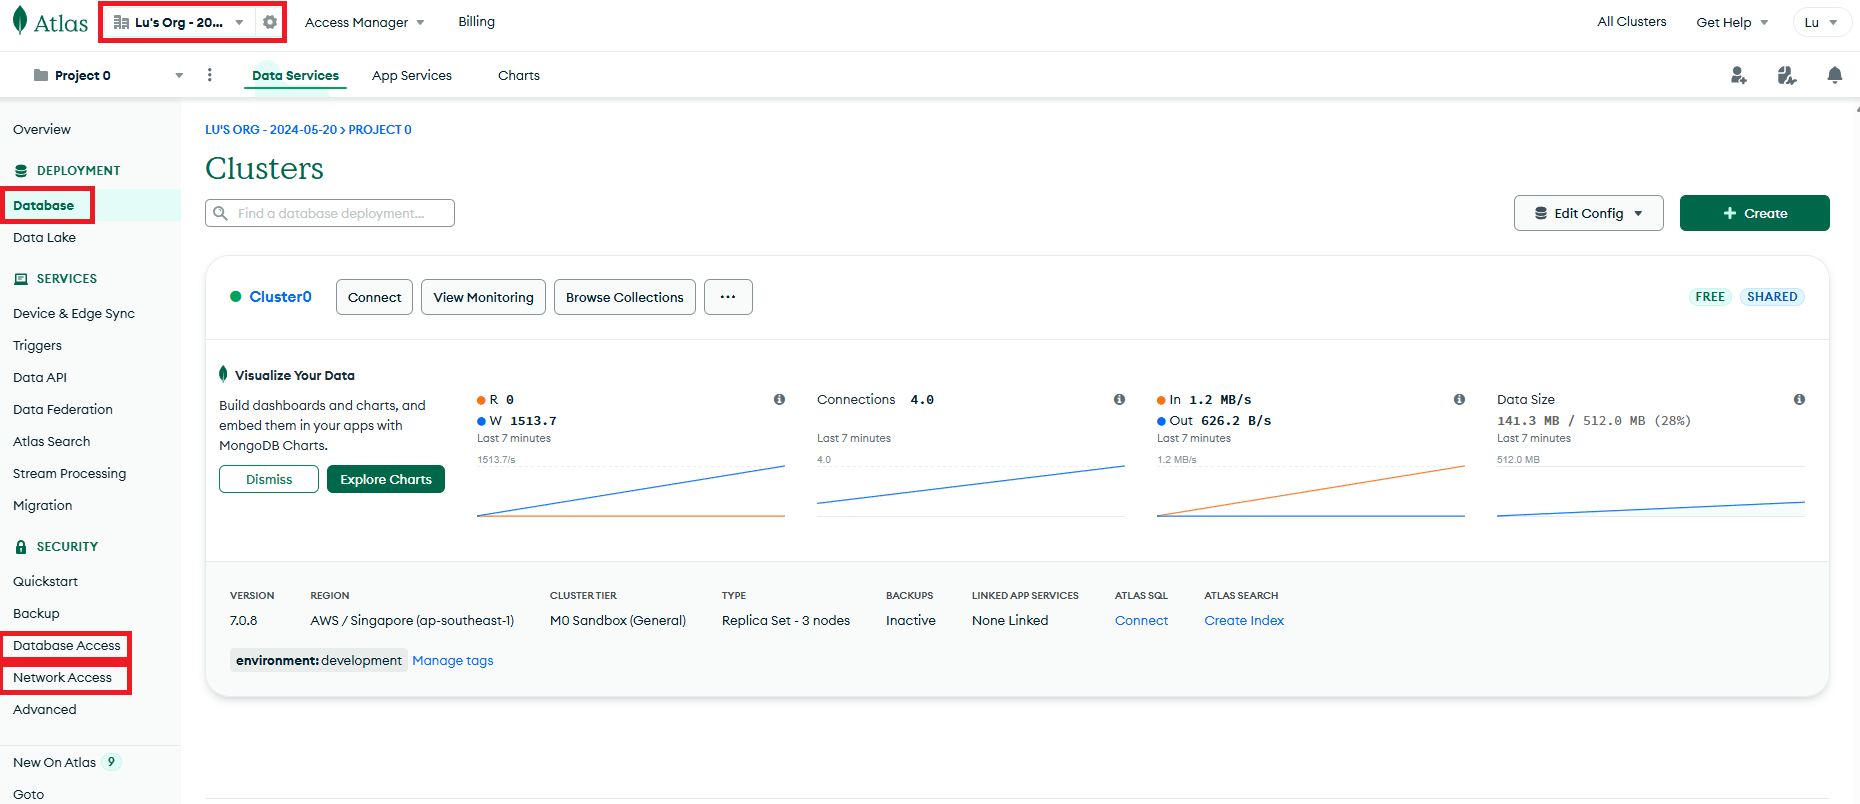
\includegraphics[width=\textwidth]{chapters/part-3/figures/atlas_dashboard.png}
	\caption{A demonstration of MongoDB Atlas dashboard.} \label{ch:database:atlasdashboard}
\end{figure}

To view collections and query for documents, click ``Browse Collections'' in Fig. \ref{ch:database:atlasdashboard} which gives Fig. \ref{ch:database:atlasdashboard2}. This sample database cluster contains multiple databases, each database with several collections, as shown by Fig. \ref{ch:database:atlasdashboard2}.

\begin{figure}[htbp]
	\centering
	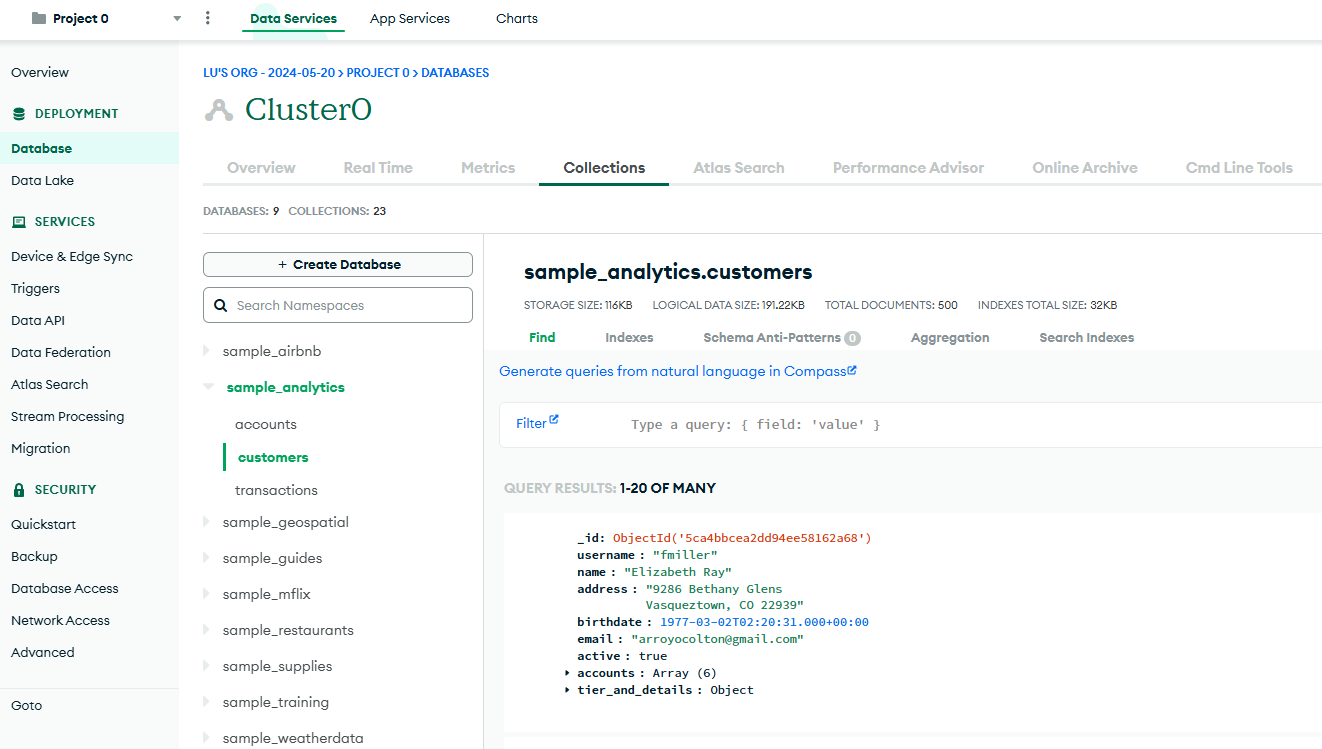
\includegraphics[width=\textwidth]{chapters/part-3/figures/atlas_dashboard_2.png}
	\caption{A demonstration of MongoDB Atlas dashboard where the databases and collections under ``\texttt{Project 0}'', ``\texttt{Cluster0}'' are browsed. Database ``\texttt{sample\_analytics}'', collection ``\texttt{customers}'' is selected. There are $500$ documents under this collection.} \label{ch:database:atlasdashboard2}
\end{figure}

\subsection{Connection String}

Database connection string allows a client to connect to a database server. MongoDB Atlas provides two connection string formats, namely the standard format and the DNS seed list format. The connection string of MongoDB Atlas can be retrieved from the dashboard by clicking ``Connect'' in Fig. \ref{ch:database:atlasdashboard}. It is possible to connect to MongoDB Atlas from:
\begin{itemize}
  \item MongoDB Shell (MongoDB's CLI)
  \item MongoDB Compass (MongoDB's desktop client GUI)
  \item User applications
\end{itemize}
Simply follow the instructions to connect to Atlas from one of the above entries. Notice that as a prerequisite, MongoDB Atlas needs to have the gateway policy to allow such connectivity.

A connection string may look like the following
\begin{lstlisting}
mongodb+srv://<username>:<password>@<server-dns>/?authSource=admin&replicaSet=myRepl
\end{lstlisting}


\section{Non-RDB Example: Redis}

Redis, short for \textit{REmote DIctionary Server}, is an open-source in-memory distributed key-value database. It is often used as a lightweight database, cache tool, or message broker. Some key features are listed below.

\begin{itemize}
\item In-memory storage. This speeds up reading and writing operations.
\item Persistence. While primarily it is an in-memory database, it also offers variety of ways to persist data on disk without compromising a lot on performance.
\item Complex data structures and associated atomic operations. Though Redis is key-value store, it supports more complex data structures than that.
\item High availability via replicas.
\item Distributed storage via horizontal partitioning.
\item Lightweight.
\end{itemize}

\section{Non-RDB Example: AllegroGraph}

Graph-based database is elsewhere introduced in details in notebook \textit{A Notebook on Probability, Statistics and Data Science} under semantic web. Check that notebook for more details. 